\section{Kaka Kamaludin}
\subsection{Soal 1}
\lstinputlisting[firstline=1, lastline=8]{src/4/1174067/Praktek/1174067_csv.py}
\subsection{Soal 2}
\lstinputlisting[firstline=8, lastline=14]{src/4/1174067/Praktek/1174067_csv.py}
\subsection{Soal 3}
\lstinputlisting[firstline=1, lastline=6]{src/4/1174067/Praktek/1174067_pandas.py}
\subsection{Soal 4}
\lstinputlisting[firstline=6, lastline=11]{src/4/1174067/Praktek/1174067_pandas.py}
\subsection{Soal 5}
\lstinputlisting[firstline=11, lastline=16]{src/4/1174067/Praktek/1174067_pandas.py}
\subsection{Soal 6}
\lstinputlisting[firstline=16, lastline=21]{src/4/1174067/Praktek/1174067_pandas.py}
\subsection{Soal 7}
\lstinputlisting[firstline=21, lastline=27]{src/4/1174067/Praktek/1174067_pandas.py}
\subsection{Soal 8}
\lstinputlisting[firstline=1, lastline=17]{src/4/1174067/Praktek/main.py}
\subsection{Soal 9}
\lstinputlisting[firstline=1, lastline=29]{src/4/1174067/Praktek/main2.py}
\subsection{keterampilan Penanganan Error}

SyntaxError: invalid token

salah dalam penulisan " import 1174067\textunderscore csv ", seharusnya "pkg = \textunderscore \textunderscore import\textunderscore \textunderscore('1174067\textunderscore csv')"

%%%%%%%%%%%%%%%%%%%%%%%%%%%%%%%%%%%%%%%%%%%%%%%%%%%%%%%%%%%%%%%%%%%%%%%%%%%%%%%%%%%%%%%%%%%%%%%%%%%%%%%%%%%%%%%%%

\section{Alfadian Owen}
\subsection{Soal 1}
Buatlah fungsi untuk membuka file csv dengan lib csv mode list
\lstinputlisting[firstline=8, lastline=14]{src/4/1174091/praktek/1174091_csv.py}

\subsection{Soal 2}
Buatlah fungsi untuk membuka file csv dengan lib csv mode dictionary
\lstinputlisting[firstline=16, lastline=21]{src/4/1174091/praktek/1174091_csv.py}

\subsection{soal 3}
Buatlah fungsi  untuk membuka csv dengan lib pandas mode list
\lstinputlisting[firstline=7, lastline=11]{src/4/1174091/praktek/1174091_pandas.py}

\subsection{Soal 4}
Buatlah fungsi untuk membuka file csv dengan lib pandas mode dictionary
\lstinputlisting[firstline=34, lastline=38]{src/4/1174091/praktek/1174091_pandas.py}

\subsection{soal 5}
Buat fungsi baru di NPM pandas.py untuk mengubah format tanggal menjadi standar dataframe
\lstinputlisting[firstline=19, lastline=22]{src/4/1174091/praktek/1174091_pandas.py}

\subsection{soal 6}
Buat fungsi baru di NPM pandas.py untuk mengubah index kolom
\lstinputlisting[firstline=24, lastline=27]{src/4/1174091/praktek/1174091_pandas.py}

\subsection{soal 7}
Buat fungsi baru di NPM pandas.py untuk mengubah atribut atau nama kolom
\lstinputlisting[firstline=29, lastline=32]{src/4/1174091/praktek/1174091_pandas.py}

\subsection{Soal 8}
Buat program main yang menggunakan library NPM csv yang membuat dan membaca file csv
\lstinputlisting[firstline=8, lastline=11]{src/4/1174091/praktek/main.py}

\subsection{Soal 9}
Buat program main2.py yang menggunakan library NPM pandas.py yang membuat dan membaca file csv
\lstinputlisting[firstline=8, lastline=20]{src/4/1174091/praktek/main.py}



%%%%%%%%%%%%%%%%%%%%%%%%%%%%%%%%%%%%%


\section{Sekar Jasmine}
\subsection{Soal 1}
\lstinputlisting[firstline=10, lastline=21]{src/4/1174075/Praktek/p_1174075_csv.py}
\subsection{Soal 2}
\lstinputlisting[firstline=23, lastline=34]{src/4/1174075/Praktek/p_1174075_csv.py}
\subsection{Soal 3}
\lstinputlisting[firstline=35, lastline=39]{src/4/1174075/Praktek/p_1174075_pandas.py}
\subsection{Soal 4}
\lstinputlisting[firstline=9, lastline=19]{src/4/1174075/Praktek/p_1174075_pandas.py}
\subsection{Soal 5}
\lstinputlisting[firstline=20, lastline=31]{src/4/1174075/Praktek/p_1174075_pandas.py}
\subsection{Soal 6}
\lstinputlisting[firstline=33, lastline=37]{src/4/1174075/Praktek/p_1174075_pandas.py}
\subsection{Soal 7}
\lstinputlisting[firstline=21, lastline=27]{src/4/1174075/Praktek/p_1174075_pandas.py}
\subsection{Soal 8}
\lstinputlisting[firstline=8, lastline=9]{src/4/1174075/Praktek/p_1174075_main.py}
\subsection{Soal 9}
\lstinputlisting[firstline=8, lastline=9]{src/4/1174075/Praktek/p_1174075_main2.py}
\subsection{keterampilan Penanganan Error}


\section{Fernando Lorencius S}
\subsection{Soal 1}
Buatlah fungsi untuk membuka file csv dengan lib csv mode list
\lstinputlisting[firstline=9, lastline=21]{src/4/1174072/Praktek/1174072_csv.py}

\subsection{Soal 2}
Buatlah fungsi untuk membuka file csv dengan lib csv mode dictionary
\lstinputlisting[firstline=25, lastline=36]{src/4/1174072/Praktek/1174072_csv.py}

\subsection{Soal 3}
Buatlah fungsi untuk membuka file csv dengan lib pandas mode list
\lstinputlisting[firstline=10, lastline=11]{src/4/1174072/Praktek/1174072_pandas.py}

\subsection{Soal 4}
Buatlah fungsi untuk membuka file csv dengan lib pandas mode dictionary
\lstinputlisting[firstline=14, lastline=16]{src/4/1174072/Praktek/1174072_pandas.py}

\subsection{Soal 5}
Buat fungsi baru untuk mengubah format tanggal menjadi standar dataframe
\lstinputlisting[firstline=19, lastline=20]{src/4/1174072/Praktek/1174072_pandas.py}

\subsection{Soal 6}
Buat fungsi baru  untuk mengubah index kolom
\lstinputlisting[firstline=23, lastline=24]{src/4/1174072/Praktek/1174072_pandas.py}

\subsection{Soal 7}
Buat fungsi baru untuk mengubah atribut atau nama kolom
\lstinputlisting[firstline=27, lastline=42]{src/4/1174072/Praktek/1174072_pandas.py}

\subsection{Soal 8}
Buat program main yang menggunakan library NPM csv yang membuat dan membaca file csv


\lstinputlisting[caption=main.py, firstline=6, lastline=10]{src/4/1174072/Praktek/main_fer.py}

\subsection{Soal 9}
Buat program main2.py yang menggunakan library NPM pandas.py yang membuat dan membaca file csv

\lstinputlisting[caption=main2.py, firstline=8, lastline=10]{src/4/1174072/Praktek/main_fer2.py}

\subsection{Keterampilan Penanganan Error}
Pada praktikum saat ini saya tidak mendapatkan error

%%%%%%%%%%%%%%%%%%%%%%%%%%%%%%%%%%%%%%%%%%%%%%%%%%%%%%%%%%%%%%%%%%%%%%%%%%

\section{Ainul Filiani}

\subsection{Keterampilan Pemograman}

\begin{enumerate}

\item Buatlah fungsi (file terpisah/library dengan nama NPM csv.py) untuk mem-buka file csv dengan lib csv mode list
Berikut adalah pemanggilan file csv dengan library csv yang menggunakan list
\lstinputlisting[firstline=10, lastline=21]{src/4/1174073/praktek/p_1174073_csv.py}
\item Buatlah fungsi (file terpisah/library dengan nama NPM csv.py) untuk mem-buka file csv dengan lib csv mode dictionary Berikut adalah pemanggilan file csv dengan library csv yang menggunakan dictionary
\lstinputlisting[firstline=23, lastline=33]{src/4/1174073/praktek/p_1174073_csv.py}
\item Buatlah fungsi (file terpisah/library dengan nama NPM pandas.py) untuk mem-buka file csv dengan lib csv mode list Berikut adalah pemanggilan file csv dengan library pandas yang menggunakan list
\lstinputlisting[firstline=8, lastline=10]{src/4/1174073/praktek/p_1174073_pandas.py}
\item Buatlah fungsi (file terpisah/library dengan nama NPM pandas.py) untuk mem-buka file csv dengan lib csv mode dictionary Berikut adalah pemanggilan file csv dengan library pandas yang menggunakan dictionary
\lstinputlisting[firstline=12, lastline=15]{src/4/1174073/praktek/p_1174073_pandas.py}
\item Buat fungsi baru di NPM pandas.py untuk mengubah format tanggal menjadi standar dataframe
Berikut penggunaan untuk merubah standar penulisan tanggal, yang mengikuti standar penulisan dari pandas.
\lstinputlisting[firstline=18, lastline=20]{src/4/1174073/praktek/p_1174073_pandas.py}
\item Buat fungsi baru di NPM pandas.py untuk mengubah index kolom
Berikut merupakan pergantian index kolom
\lstinputlisting[firstline=22, lastline=24]{src/4/1174073/praktek/p_1174073_pandas.py}
\item Buat fungsi baru di NPM pandas.py untuk mengubah atribut atau nama kolom berikut merupakan penggunaan untuk merename atribut yang digunakan, atau merubah nama header 0
\lstinputlisting[firstline=27, lastline=31]{src/4/1174073/praktek/p_1174073_pandas.py}
\item Buat program main.py yang menggunakan library NPM csv.py yang membuat dan membaca 
file csv
\lstinputlisting[firstline=7, lastline=8]{src/4/1174073/praktek/p_1174073_pandas.py}
\item Buat program main2.py yang menggunakan library NPM pandas.py yang mem- buat dan membaca 
file csv
\lstinputlisting[firstline=8, lastline=9]{src/4/1174073/praktek/p_1174073_main2.py}

\end{enumerate}
%%%%%%%%%%%%%%%%%%%%%%%%%%%%%%%%%%%%%%%%%%%%%%%%%%%%%%%%%%%%%%%%%%%%%%%%%%%%%
\section{Alvan Alvanzah|1174077}
\subsection{Ketrampilan Pemrograman}

\begin{enumerate}
    \item Buatlah  fungsi  (file  terpisah/library  dengan  nama  NPMcsv.py)  untuk  mem-buka file csv dengan lib csv mode list
    \lstinputlisting[firstline=11, lastline=15]{src/4/1174077/praktek/1174077_csv.py}
    
    \item Buatlah  fungsi  (file  terpisah/library  dengan  nama  NPMcsv.py)  untuk  mem-buka file csv dengan lib csv mode dictionary
    \lstinputlisting[firstline=18, lastline=22]{src/4/1174077/praktek/1174077_csv.py}
    
    \item Buatlah fungsi (file terpisah/library dengan nama NPMpandas.py) untuk mem-buka file csv dengan lib pandas mode list
    \lstinputlisting[firstline=11, lastline=13]{src/4/1174077/praktek/1174077_pandas.py}
    
    \item Buatlah fungsi (file terpisah/library dengan nama NPMpandas.py) untuk mem-buka file csv dengan lib pandas mode dictionary
    \lstinputlisting[firstline=16, lastline=19]{src/4/1174077/praktek/1174077_pandas.py}
    
    \item Buat fungsi baru di NPMpandas.py untuk mengubah format tanggal menjadistandar dataframe
    \lstinputlisting[firstline=22, lastline=24]{src/4/1174077/praktek/1174077_pandas.py}
    
    \item Buat fungsi baru di NPMpandas.py untuk mengubah index kolom
    \lstinputlisting[firstline=27, lastline=30]{src/4/1174077/praktek/1174077_pandas.py}
    
    \item Buat fungsi baru di NPMpandas.py untuk mengubah atribut atau nama kolom
    \lstinputlisting[firstline=33, lastline=36]{src/4/1174077/praktek/1174077_pandas.py}
    
    \item Buat program main.py yang menggunakan library NPMcsv.py yang membuat dan membaca file csv
    \lstinputlisting[firstline=8, lastline=13]{src/4/1174077/praktek/main.py}
    
    \item Buat program main2.py yang menggunakan library NPMpandas.py yang membuat dan membaca file csv
    \lstinputlisting[firstline=8, lastline=13]{src/4/1174077/praktek/main2.py}
\end{enumerate}

\textbf{Kode Program}
\begin{figure}[!htbp]
	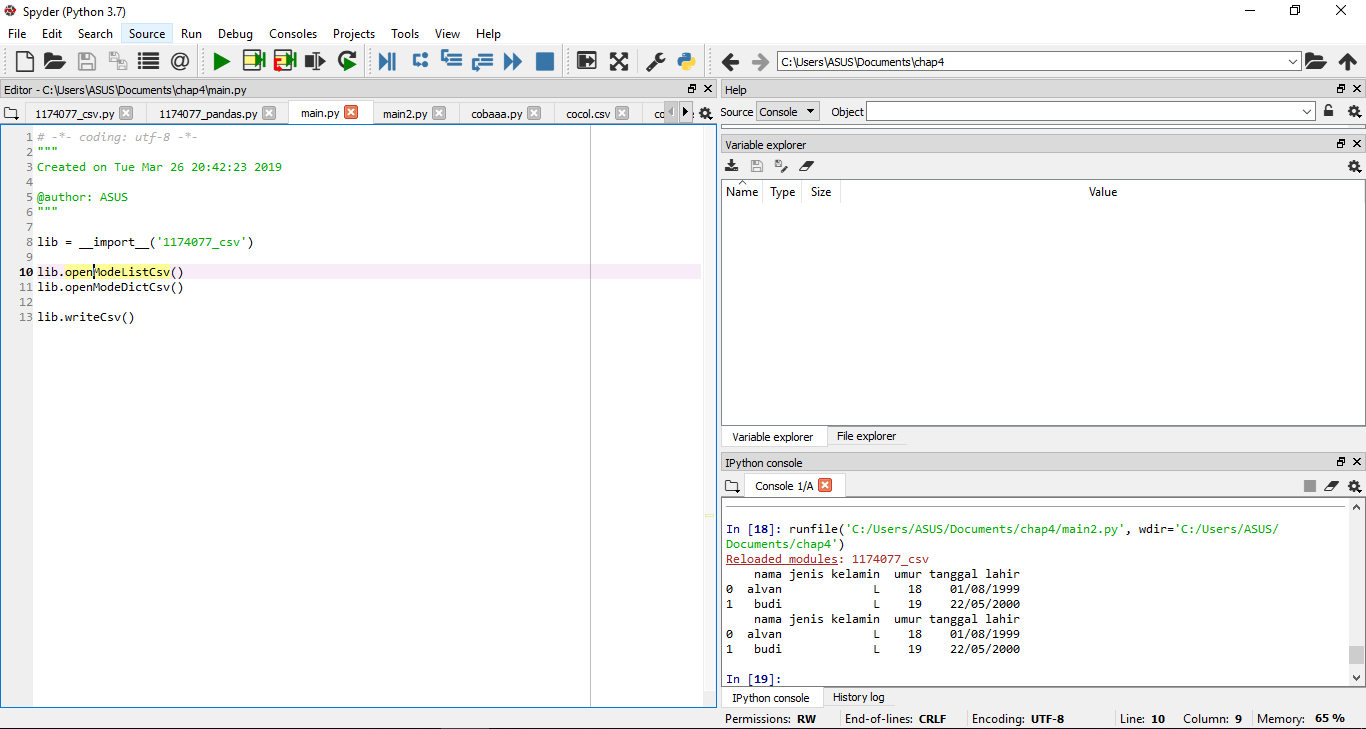
\includegraphics[width=10cm]{figures/4/1174077/praktek/mainpy.png}
	\centering
\end{figure}
\begin{figure}[!htbp]
	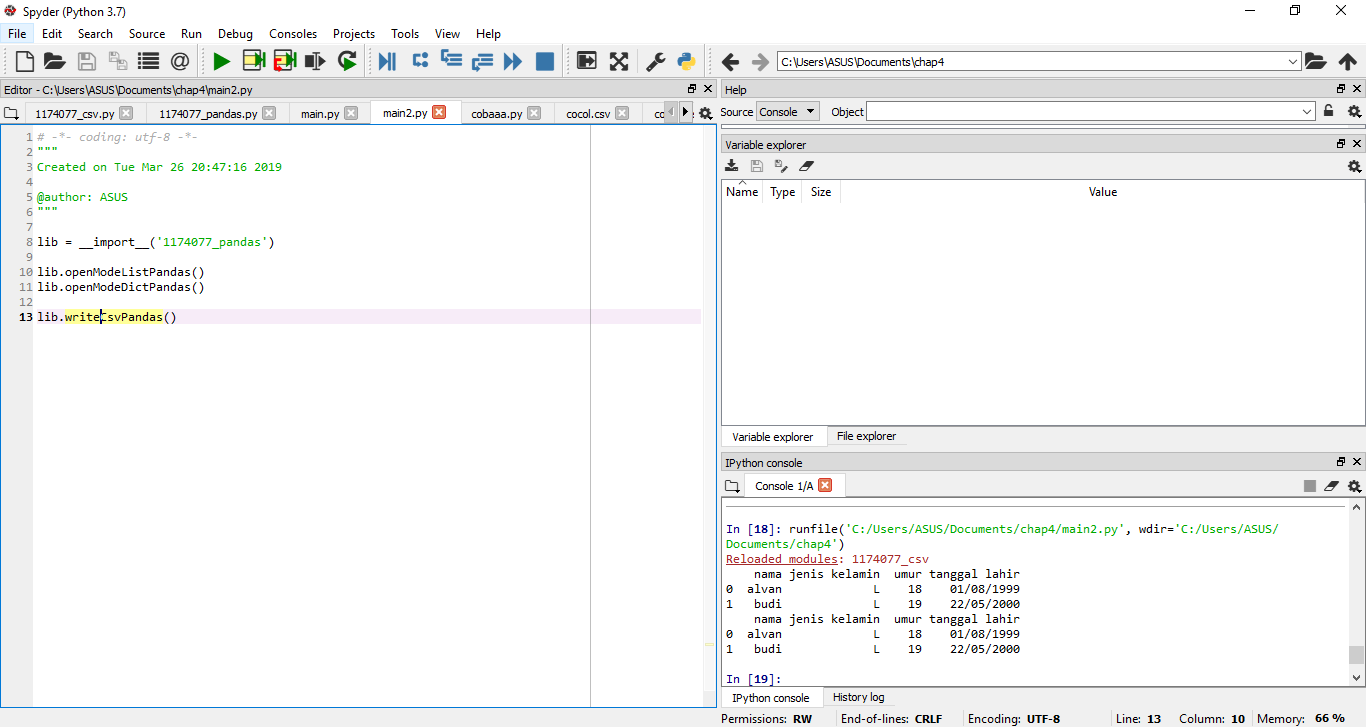
\includegraphics[width=10cm]{figures/4/1174077/praktek/main2py.png}
	\centering
\end{figure}
\begin{figure}[!htbp]
	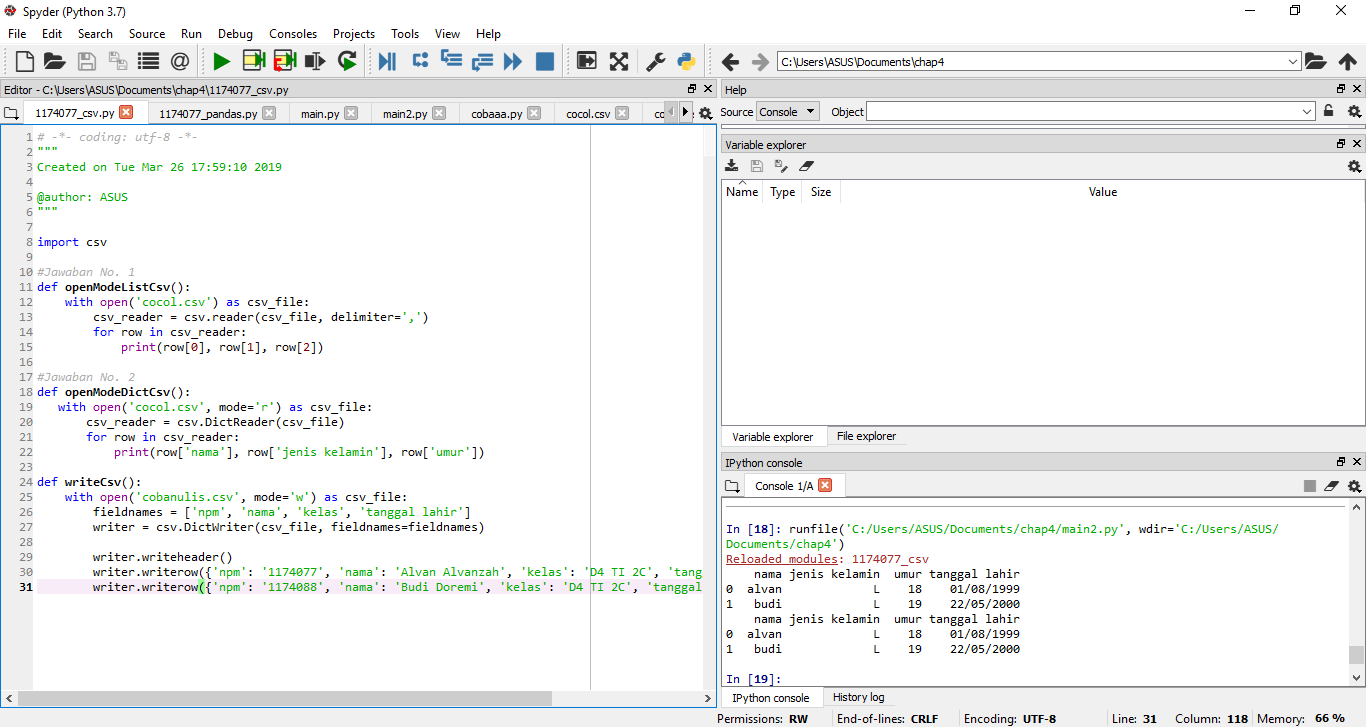
\includegraphics[width=10cm]{figures/4/1174077/praktek/csv.png}
	\centering
\end{figure}
\begin{figure}[!htbp]
	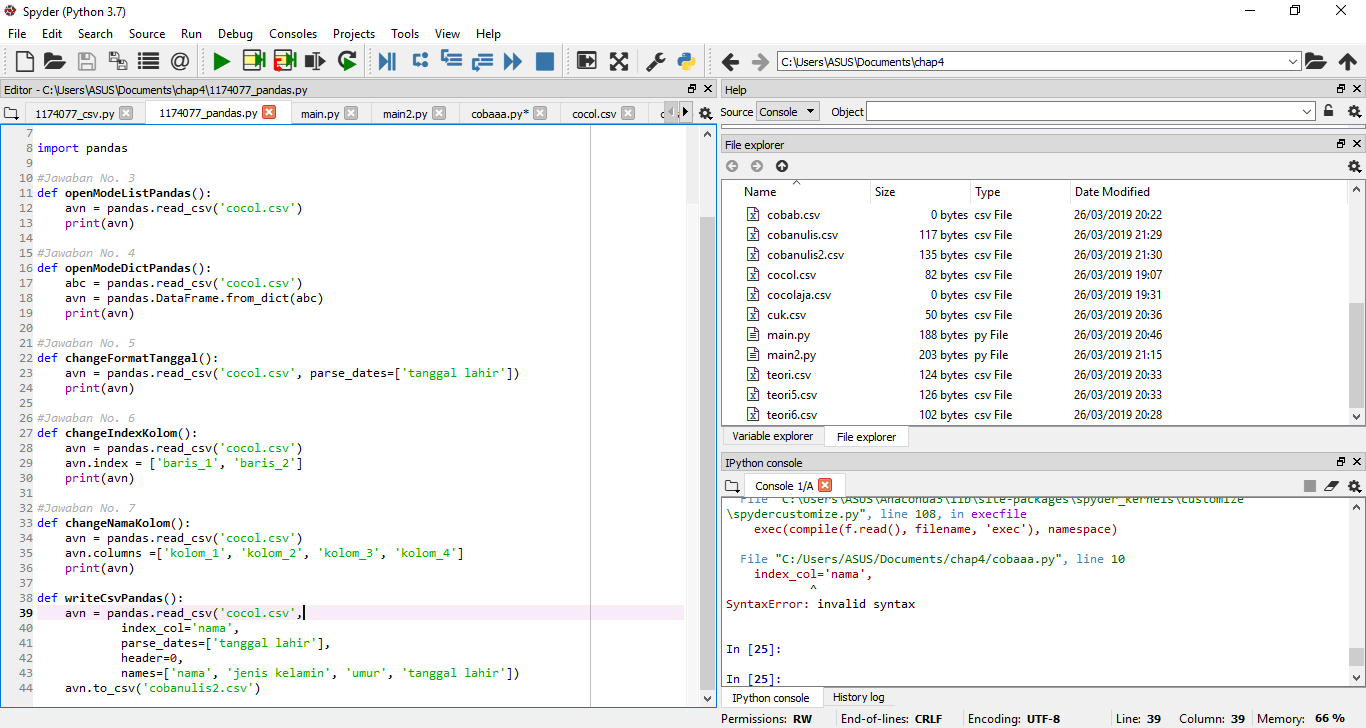
\includegraphics[width=10cm]{figures/4/1174077/praktek/pandas.png}
	\centering
\end{figure}
%%%%%%%%%%%%%%%%%%%%%%%%%%%%%%%%%%%%%%%%%%%%%%%%%%%%%%%%%%%%%%%%%%%%%%%%%%%%%%%%%%%%%%%%%%%%%%%%%%%%

\section{Muhammad Abdul Gani Wijaya}
\subsection{No 1}
Buatlah  fungsi  (file  terpisah/library  dengan  nama  NPMcsv.py)  untuk  membuka file csv dengan lib csv mode list.

\lstinputlisting[caption = Fungsi membuka file CSV dengan lib CSV mode list., firstline=8, lastline=19]{src/4/1174071/Praktek/1174071_csv.py}

\subsection{No 2}
Buatlah  fungsi  (file  terpisah/library  dengan  nama  NPMcsv.py)  untuk  membuka file csv dengan lib csv mode dictionary.

\lstinputlisting[caption =  Fungsi membuka file CSV dengan lib CSV mode dictionary., firstline=21, lastline=30]{src/4/1174071/Praktek/1174071_csv.py}

\subsection{No 3}
Buatlah fungsi (file terpisah/library dengan nama NPMpandas.py) untuk membuka file csv dengan lib pandas mode list.

\lstinputlisting[caption =  Fungsi membuka file CSV dengan lib Pandas mode list., firstline=9, lastline=14]{src/4/1174071/Praktek/1174071_pandas.py}

\subsection{No 4}
Buatlah fungsi (file terpisah/library dengan nama NPMpandas.py) untuk membuka file csv dengan lib pandas mode dictionary.

\lstinputlisting[caption =  Fungsi membuka file CSV dengan lib Pandas mode dictionary., firstline=16, lastline=22]{src/4/1174071/Praktek/1174071_pandas.py}

\subsection{No 5}
Buat fungsi baru di NPMpandas.py untuk mengubah format tanggal menjadi standar dataframe.

\lstinputlisting[caption =  Fungsi mengubah format tanggal menjadi standar dataframe., firstline=24, lastline=29]{src/4/1174071/Praktek/1174071_pandas.py}

\subsection{Soal 6}
Buat fungsi baru di NPMpandas.py untuk mengubah index kolom.

\lstinputlisting[caption =  Fungsi mengubah index kolom., firstline=31, lastline=37]{src/4/1174071/Praktek/1174071_pandas.py}

\subsection{Soal 7}
Buat fungsi baru di NPMpandas.py untuk mengubah atribut atau nama kolom.

\lstinputlisting[caption =  Fungsi untuk mengubah atribut atau nama kolom., firstline=26, lastline=30]{src/4/1174071/Praktek/1174071_pandas.py}

\subsection{Soal 8}
Buat program main.py yang menggunakan library NPMcsv.py yang membuat dan membaca file csv.

\lstinputlisting[caption =  Membuat dan membaca file CSV menggunakan library 1174071pandas., firstline=8, lastline=13]{src/4/1174071/Praktek/main.py}

\subsection{Soal 9}
Buat program main2.py yang menggunakan library NPMpandas.py yang membuat dan membaca file csv.

\lstinputlisting[caption = Membuat dan mmebaca file CSV menggunakan library 1174071pandas., firstline=8, lastline=13]{src/4/1174071/Praktek/main2.py}

\subsection{Kode Program Praktek}
\begin{figure}[ht]
	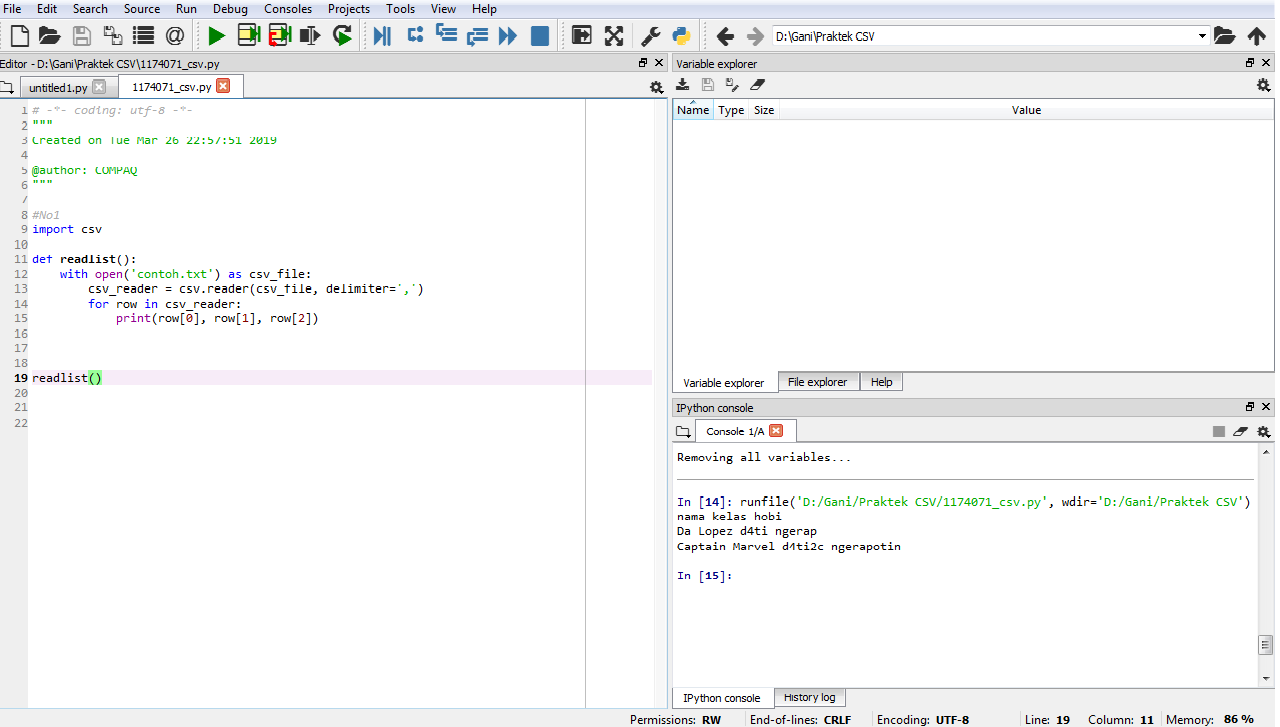
\includegraphics[width=9cm]{figures/4/1174071/Praktek/1174071_csv1.png}
	\centering
\end{figure}
\begin{figure}[ht]
	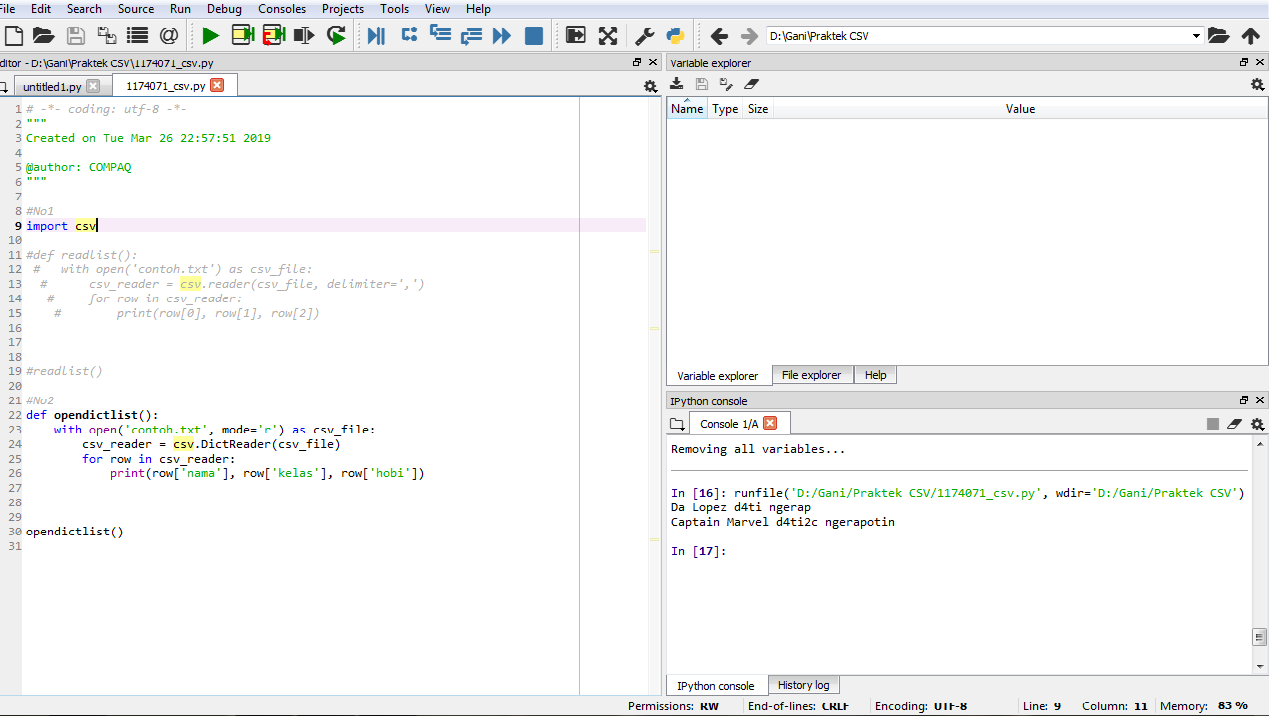
\includegraphics[width=10cm]{figures/4/1174071/Praktek/1174071_csv2.png}
	\centering
\end{figure}
\begin{figure}[ht]
	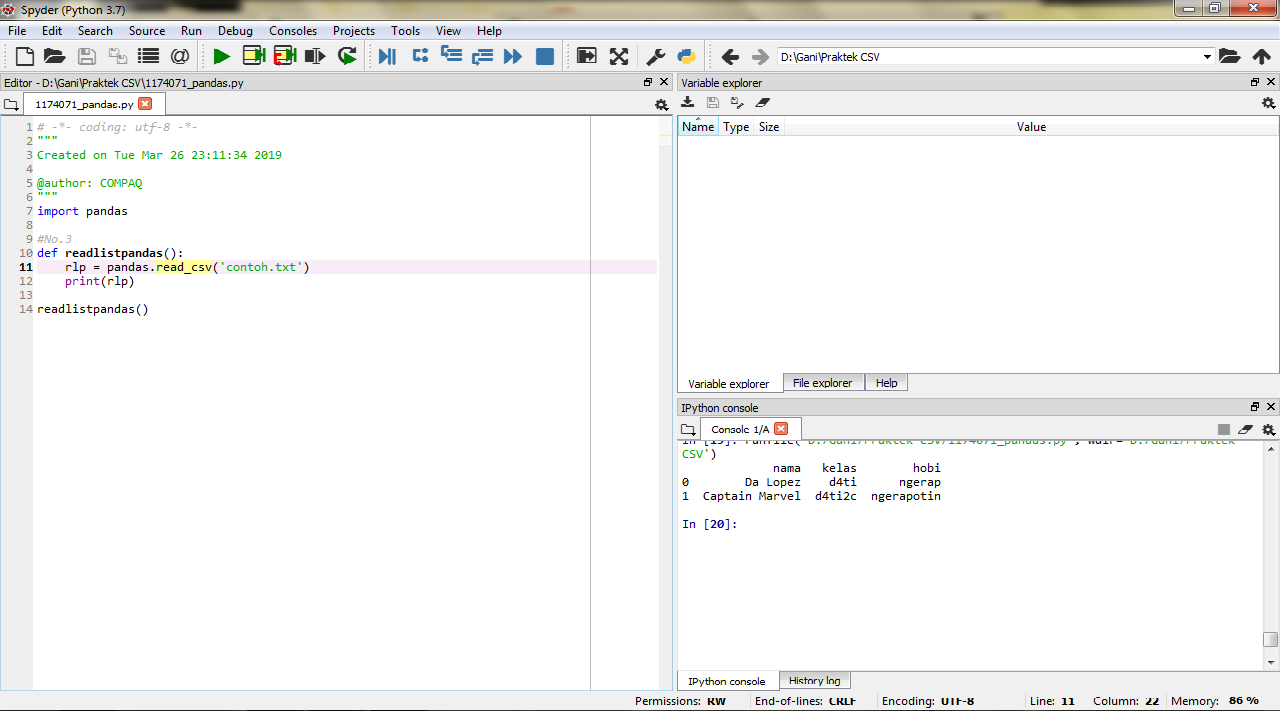
\includegraphics[width=10cm]{figures/4/1174071/Praktek/1174071_pandas3.png}
	\centering
\end{figure}
\begin{figure}[ht]
	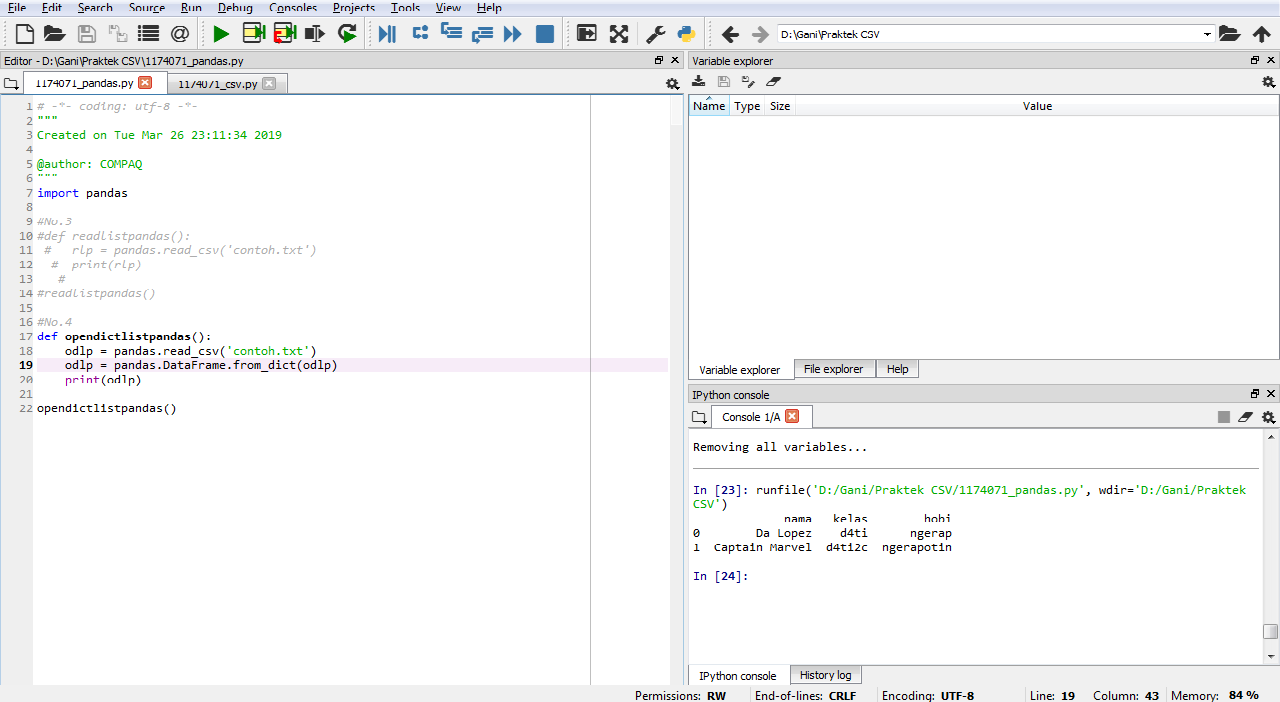
\includegraphics[width=9cm]{figures/4/1174071/Praktek/1174071_pandas4.png}
	\centering
\end{figure}
\begin{figure}[ht]
	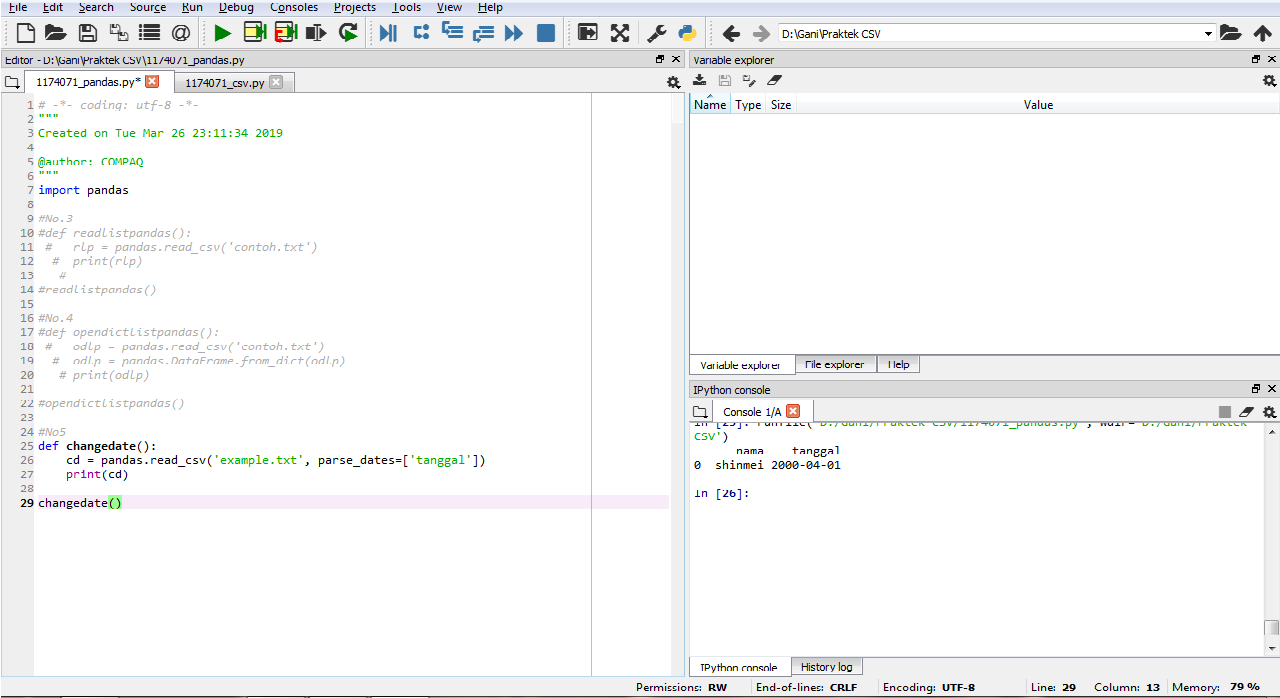
\includegraphics[width=10cm]{figures/4/1174071/Praktek/1174071_pandas5.png}
	\centering
\end{figure}
\begin{figure}[ht]
	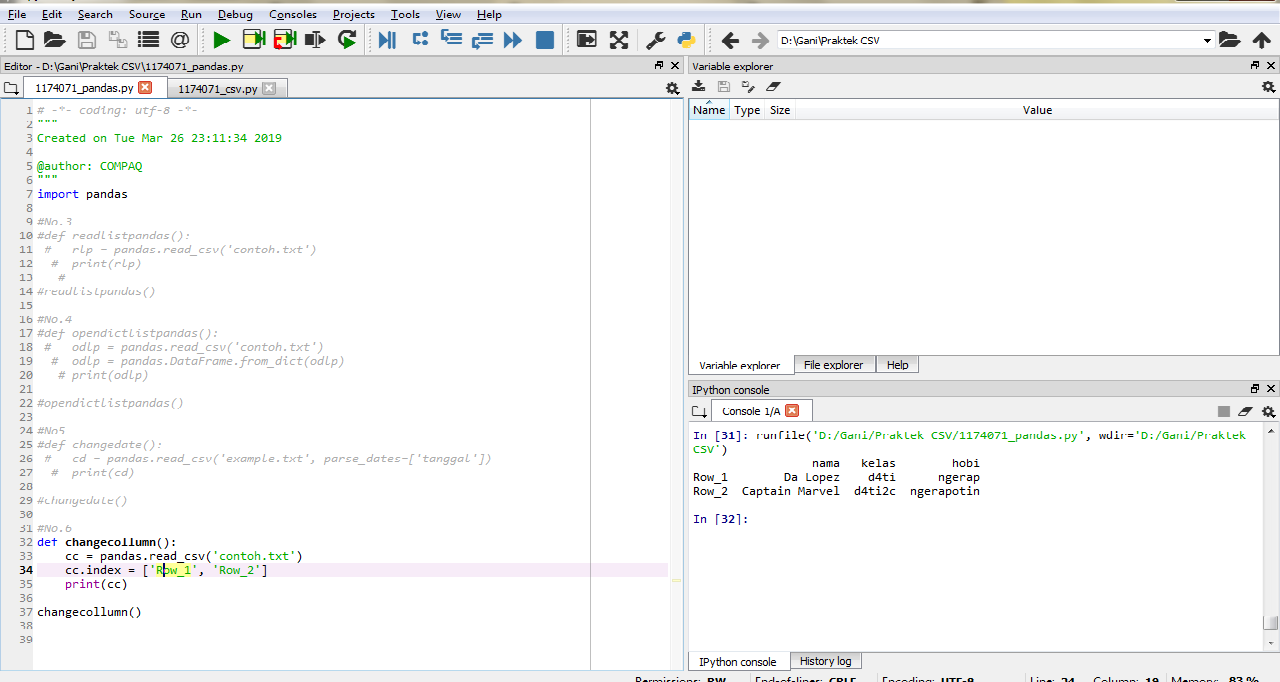
\includegraphics[width=10cm]{figures/4/1174071/Praktek/1174071_pandas6.png}
	\centering
\end{figure}
\begin{figure}[ht]
	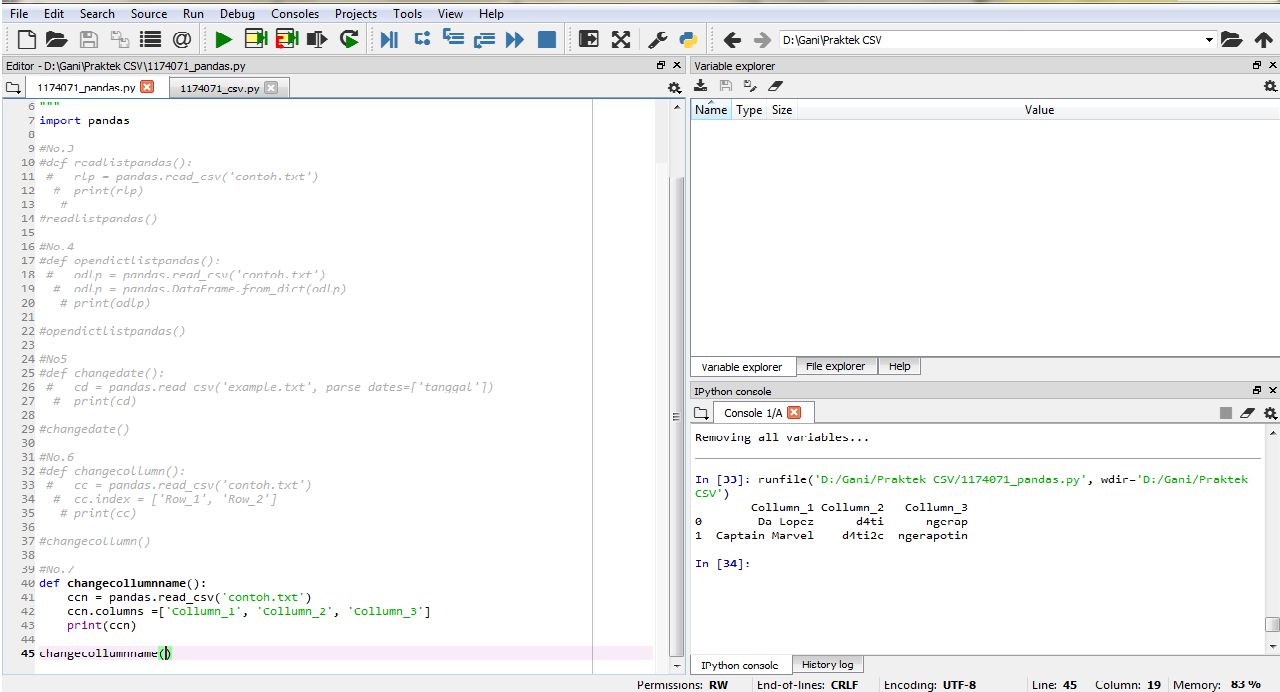
\includegraphics[width=10cm]{figures/4/1174071/Praktek/1174071_pandas7.png}
	\centering
\end{figure}
\begin{figure}[ht]
	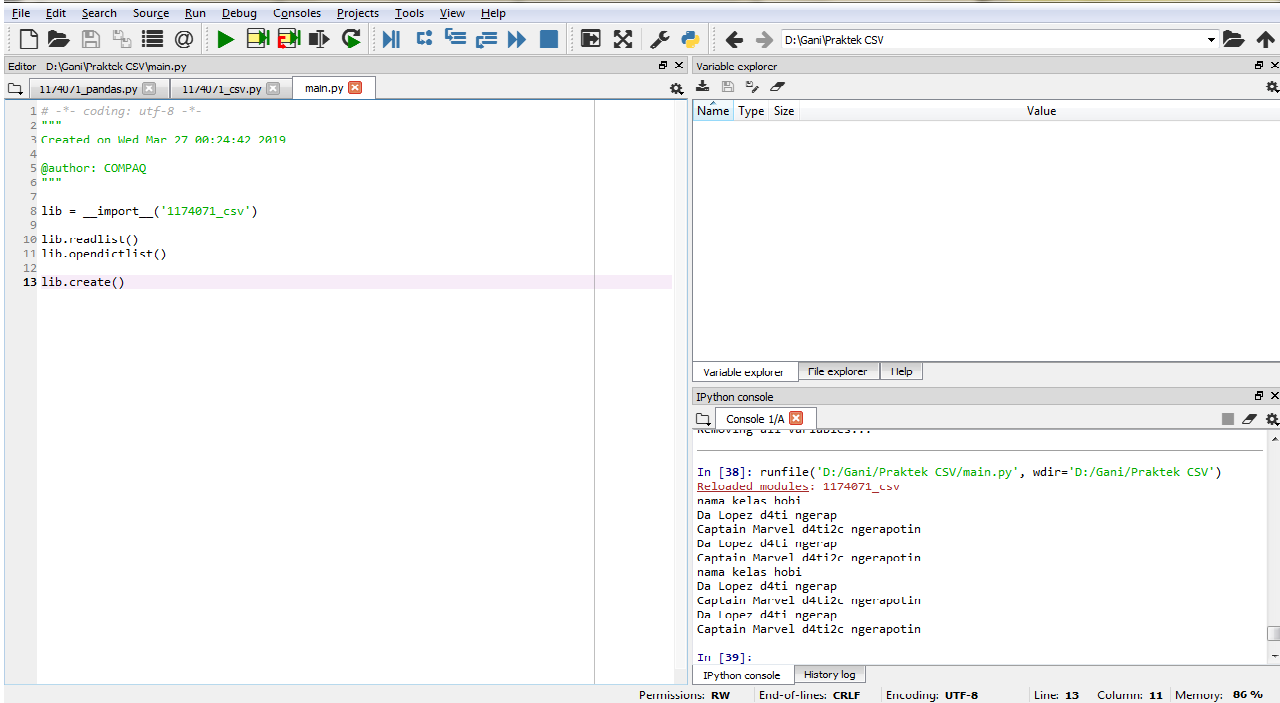
\includegraphics[width=10cm]{figures/4/1174071/Praktek/1174071_main8.png}
	\centering
\end{figure}
\begin{figure}[ht]
	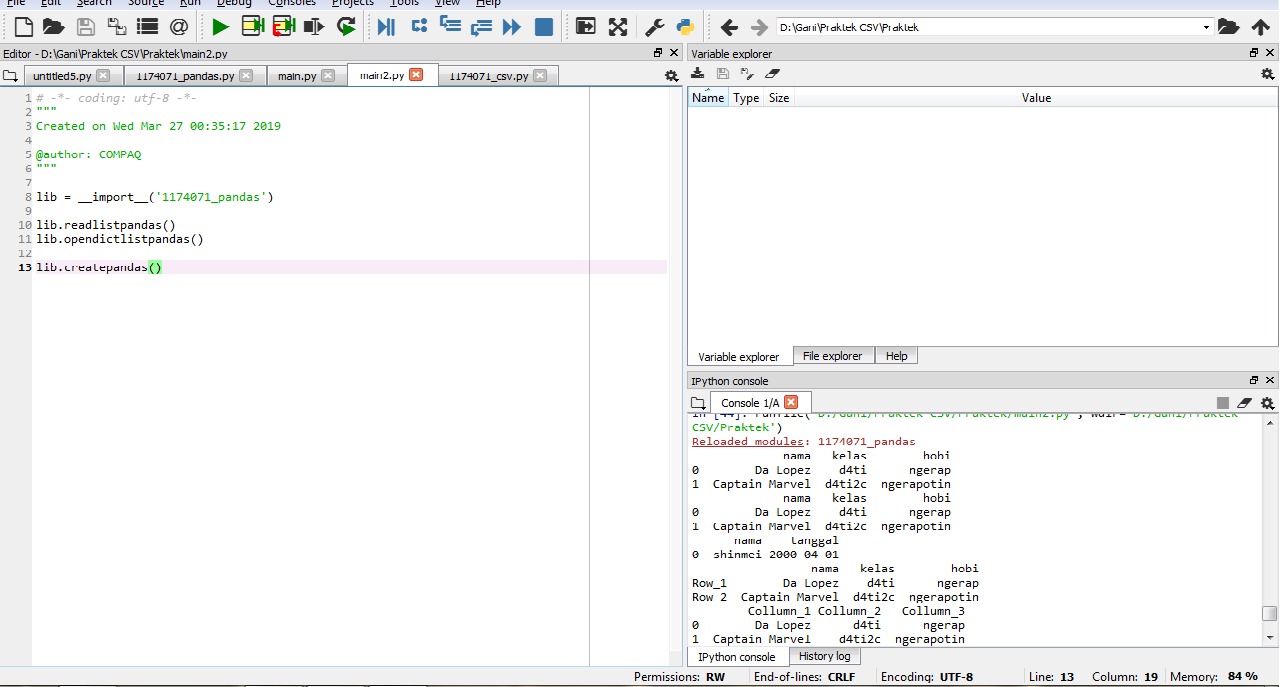
\includegraphics[width=10cm]{figures/4/1174071/Praktek/1174071_main9.png}
	\centering
\end{figure}


%%%%%%%%%%%%%%%%%%%%%%%%%%%%%%%%%%%%%%%%%%%%%%%%%%%%%%%%%%%%%%%%%%%%%%%%%%%%%%%%%%%%%%%%%%%%%%%%%%%%%
